\documentclass[main.tex]{subfiles}
\begin{document}
\chapter{数值实验}\label{chp:experiments}

(\ref{eq:Multi}) 和 (\ref{eq:group}) 都可以写成矩阵的形式
\begin{align}\label{eq:MatrixLasso}
  \min_{C} \; \|C\|_{\Omega}+\frac{\lambda}{2}\|X-XC\|_F^2 \quad
  \text{s.t.} \;\quad\mathrm{diag}(C)=0, \text{or} \quad \mathrm{B-diag}(C)=0,
\end{align}
其中$\|\dot\|_{\Omega}$ 为某个与指标集集合$\Omega$有关的凸范数,
$\mathrm{B-diag}(C)$是指将$C$按照类别排序后,同类的对角块。(\ref{eq:MatrixLasso})
可以用ADMM算法求解~\cite{boyd2011admm}。
\section{ADMM 算法}
简单起见,我们将$\mathrm{diag}()$和$\mathrm{B-diag}$统一写成
$\mathrm{diag}()$,并把(\ref{eq:MatrixLasso})改写成下面的等价形式
\begin{align}\label{eq:MatrixLasso_modify}
  \min_{C} \; &\|C\|_{\Omega}+\frac{\lambda}{2}\|X-XJ\|_F^2 \\
  \text{s.t.} \;&\quad J=C-\mathrm{diag}(C).
\end{align}

在 Lagrangian 上增加一个等价的二次惩罚项得到增广Lagrangian
\begin{align*}
  \mathcal{L}=& \|C\|_{\Omega}+\frac{\lambda}{2}\|X-XJ\|_F^2 
  + \frac{\mu}{2}\|J-C+\mathrm{diag}(C)\|_F^2
  +tr(\Lambda^T(J-C+\mathrm{diag}(C))),
\end{align*}
其中$\Lambda$是对偶变量,$\mu$是给定参数。为了交替优化
$J$, $C$ 和 $\Lambda$ 直到收敛,需要求解 $\partial \mathcal{L}/\partial J=0$
和 $\partial \mathcal{L}/\partial C=0$。
虽然目标函数关于 $C$ 不可导,但极值可以用拓展的 Soft-Threshold
算子求得~\cite{donoho1995noising}。先定义
\begin{align*}
  S_a(x) = \begin{cases}
    \mathrm{0} & \|x\|_2 \le a, \\
    (\|x\|_2 - a) \frac{x}{\|x\|_2} & \|x\|_2 > a.
  \end{cases}
\end{align*}
其中$a$为给定正数,$x$为任意向量.
再定义作用在$\R^{n\times n}$上的变换
$\mathrm{SoftThresh}_a()$,
对于multitasking情形,我们将矩阵的每一个行向量$x$,按照
类别拆分成$\{x_I\}$,分别变成$S_a(x_I)$。
对于Group LASSO就是如此作用于列向量。
于是有算法~\ref{alg:MatrixSSC}.
注意到 $(\lambda X^TX+\mu I)$
的逆能被预先算好,这样每次迭代的时间就主要花在计算矩阵乘法上。 

\begin{algorithm}[tb]
  \caption{Group-LASSO-SSC}
  \label{alg:MatrixSSC}
  \begin{algorithmic}
    \State {\bfseries 输入:}
    $n$ 个样本点 $x_1,\ldots,x_n$,它们组成了数据矩阵$X\in \R^{d\times n}$,类别信息$\Omega$,参数$\lambda$ 和 $\mu$
    \State 初始化 $C=0$, $J=0$, $\Lambda=0$
    \While{未收敛}
    \State{1. } 更新 $J$ 
    $$J=(\lambda X^TX+\mu I)^{-1}(\lambda X^TX+\mu C-\Lambda).$$
    \State{2. } 更新 $C$
    $$ C^{'}=\mathrm{SoftThresh}_{\frac{1}{\mu}}\left(J+\Lambda/\mu\right), $$
    $$ C=C^{'}-\mathrm{diag}(C^{'}).$$
    \State{3. } 更新 $\Lambda$
    $$\Lambda=\Lambda+\mu(J-C)$$
    \EndWhile
    \State {\bfseries 输出:} 样本点的邻接矩阵$W=|C|+|C|^T$
  \end{algorithmic}
\end{algorithm}

\section{合成数据}

\section{运动分割}
\begin{figure}[tb]
  \centering
  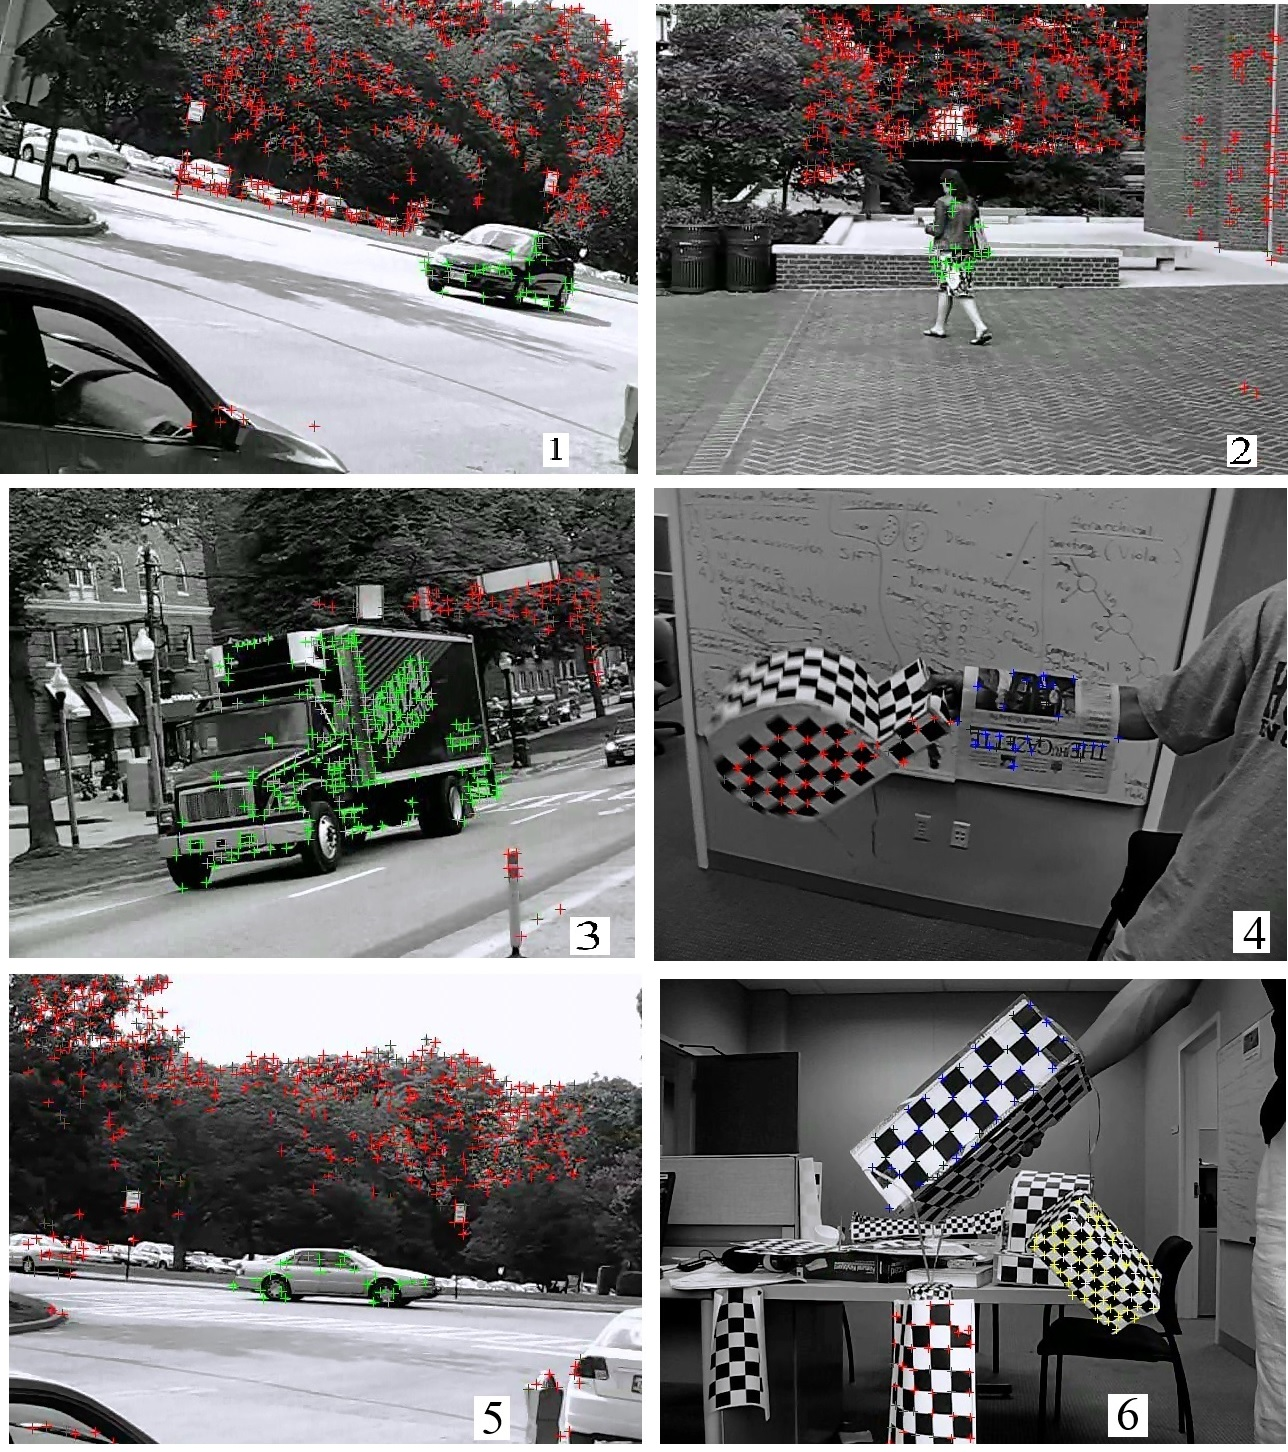
\includegraphics[width=0.8\textwidth]{pics/newsnp.jpg}
  \caption{Hopkins155 中的视频 }
  \label{snpsht}
\end{figure}
我们将GL-SSC 和 Multi-SSC 用于运动分割,即Hopkins155 \cite{tron2007benchmark}
数据集上。 Hopinks 155 包含155个视频,分别记录了棋盘,车辆和行人的运动。每个
视频中有2 或 3 个物体,我们的任务是将它们的轨迹点分开。
图~\ref{snpsht}
展示了数据集中的某些帧,一个标记的点在多帧中的位置组成了高维空间中的一个样本点。
由于同一个运动刚体上的点在一个低维子空间中,运动分割可以转化为子空间聚类问题。
我们分别比较SSC,LRR,GL-SSC,Multi-SSC四种算法的效果,结果如表~\ref{tab:hopkins}
\footnote{SSC 和 LRR 算法的MATLAB代码下载自 http://vision.jhu.edu/code/ 和
https://sites.google.com/site/guangcanliu/ 。}。
\begin{table}[h]
  \label{tab:hopkins}
  \centering
  \begin{tabular}{|c | c |c| c | c | c | c | }
	\hline
	L & 算法 & SSC & LRR & GL-SSC & Multi-SSC \\
	\hline  \hline
	2 & 1.52 & 2.13& 1.43 & 1.36 \\
	\hline
	3 & 0 & 0 & 0  &  1 & 4 & 504 \\
	\hline
  \end{tabular}
  \caption{SSC,LRR,GL-SSC和Multi-SSC在Hopkins
  155上的聚类错误率比较(越低越好,单位\%)}
\end{table}

\section{人脸聚类}

根据 \cite{basri2003lambertianface} 不同光照下的人脸图片近似
分布在9维线性子空间。Extended YaleB \cite{lee2005extendedyalb}
是一个人脸图片集,包括了38人,64种不同光照下的照片,它们没有
未经处理时,人脸在照片中的位置不尽相同,作者提供了手动裁剪和
对齐的版本,如图~\ref{fig:yaleb}所示。
\begin{figure}[h]
  \centering
  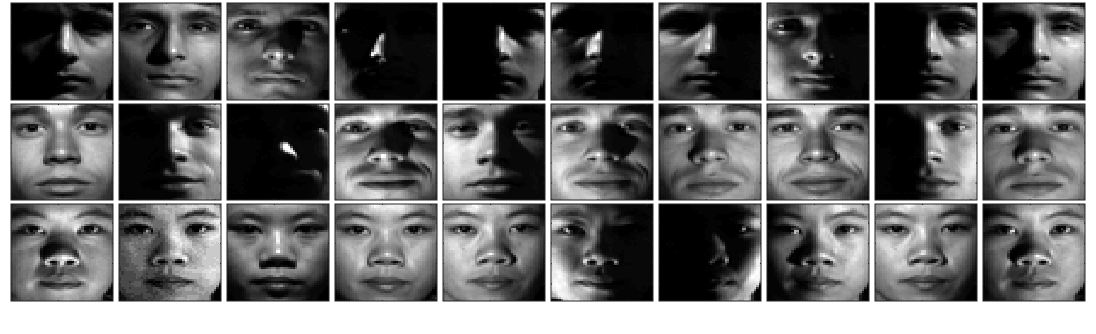
\includegraphics[width=0.8\textwidth]{pics/yaleb}
  \caption{3人在不同光照下的面部照片,注意这经过手动对齐}
  \label{fig:yaleb}
\end{figure}
\end{document}
